\documentclass{article}

\usepackage[utf8]{inputenc}
\usepackage{amsmath}
\usepackage{tabularx}
\usepackage{graphicx}
\usepackage{tikz}
\usetikzlibrary{shapes.geometric, arrows}
\usepackage{listings}

% Tickz Block Styles
\tikzstyle{decision} = [diamond, draw,
    text width=4.5em, text badly centered, node distance=3cm, inner sep=0pt]
\tikzstyle{block} = [rectangle, draw,
    text width=5em, text centered, rounded corners, minimum height=4em]
\tikzstyle{focus} = [rectangle, draw,
    text width=8em, text centered, rounded corners, minimum height=4em]
\tikzstyle{line} = [draw, -latex']
\tikzstyle{cloud} = [draw, ellipse, node distance=3cm,
    minimum height=2em]
    

\title{Programmazione\\ \large\textbf{Amato Flora} \\ a.a. 2023-2024}

\author{\textbf{Author}\\ Alessio Romano}

\begin{document}
\maketitle

\newpage
\tableofcontents
\newpage

\section{Sottoprogrammi}
I \textbf{sottoprogrammi} costituiscono un meccanismo di astrazione procedurale (astrazione sul controllo).\\
Si tratta di sezione di codice che non vengono eseguite autonomamente una volta implementate, ma su chiamata di un programma esterno. Essi svologono funzioni di utilitá generale (ex. librerie), o semplicemente aiutano a sviluppare codice ben strutturato e modulare. Utilizzare sottoprogrammi comporta vari vantaggi
\begin{itemize}
    \item Suddivisione del programma in unitá significative
    \item Testo di ogni unitá piú breve
    \item Riutilizzo del codice
    \item Migliore leggibilitá
    \item Sviluppo top-down del software
\end{itemize}
\subsection{Funzionamento di un sottoprogramma}
    Ai sottoprogrammi vengono assegnate determinate responsabilitá, che includono la risoluzione di un sottoproblema. I sotto programmi hanno due caratteristiche principali
    \begin{itemize}
        \item Un \textbf{nome} per effettuare la chiamata da qualunque punto del programma chiamante
        \item Un unico \textbf{entry-point} ed  un unico \textbf{exit-point} (secondo i principi della programmazione strutturata).
    \end{itemize}
    Il flusso di controllo é ceduto dal modulo chiamante al sottoprogramma da una istruzione di \textbf{chiamata}
    \begin{figure}[h]
        \begin{center}
            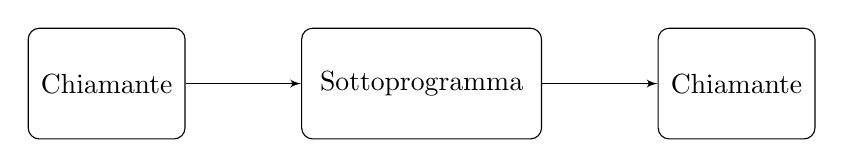
\begin{tikzpicture}[node distance=1cm]
                \node [block] at (0,0) (call) {Chiamante};
                \node [focus] at (4,0) (func) {Sottoprogramma};
                \node [block] at (8,0) (return) {Chiamante};
                \path [line] (call) -- (func);
                \path [line] (func) -- (return);
            \end{tikzpicture}
            \caption{chiamata a sottoprogramma}
        \end{center}    
    \end{figure}
    L'interazione tra il sottoprogramma e il programma chiamante avviene mediante uno scambio di dati. I dati possono essere di ingresso, di uscita o di ingresso/uscita.\\
    Lo scambio avviene mediante paramentri, ne esistono di due tipi:
    \begin{itemize}
        \item \textbf{Paramentri formali}: nomi delle variabili passate alla funzione
        \item \textbf{Parametri attuali}: valori delle variabili passate alla funzione
    \end{itemize}
    I parametri formali e attuali devono coincidere in numero, posizione e tipo.
    \begin{lstlisting}[language=c++]
        int b;
        stampa(b);
        // b parametro effettivo
    \end{lstlisting}    
    \begin{lstlisting}[language=c++]
        void stampa (const int x){
            // x parametro formale
            cout << x;
        }
    \end{lstlisting}    
    Quando si esegue una chiamata ad un sottoprogramma, per la \textbf{regola della sostituzione}, l'effetto che si ottiene é l'esecuzione del sottoprogramma con la sostituzione di ciascun parametro effettivo a ciascun parametro formale
    \subsection{Tipi di sottoprogrammi e astrazione sul controllo}
    Definiamo 2 diversi tipi di sottoprogrammi
    \begin{itemize}
        \item \textbf{Funzioni}: esprimono l'astrazione matematica di una funzione, calcolano un risultato valutato a partire dai valori che vengono forniti. Una funzione ritorna un unico valore di tipo atomico attraverso l'istruzione \textit{return}
        \item \textbf{Procedure}: esprimono l'astrazione di un insieme di azioni che producono degli "effetti" ma non "ritornano" alcun risultato
    \end{itemize}
    I sottoprogrammi in genere, implementano un \textbf{astrazione sul controllo}, ossia possono essere considerate \textbf{black box}.\\
    Essi svolgono un compito, offrendo un servizio a chi li utilizza, ma chi chiama il sottoprogramma non ha visibilitá dell'implementazione di quest'ultimo.\\L'interazione tra sottoprogramma ed ambiente esterno avviene mediante una precisa interfaccia costituita dall'intestazione.
    \subsection{Interfaccia}
    L'interfaccia di un sottoprogramma deve specificare
    \begin{itemize}
        \item Il nome del sottoprogramma (deve essere significativo della funzionalitá di quest'ultimo)
        \item I parametri di input
        \item I parametri di output
    \end{itemize}
        \begin{lstlisting}[language=c++]
            int incr(int); // intestazione

            incr(x){
                x++
                return x
            }
    \end{lstlisting}    
    \subsection{Modi di scambio dei paramentri}
    Esistono diversi modi per effettuare lo scambio tra parametri effettivi e paramentri globali.
    \begin{itemize}
        \item \textbf{passaggio per valore}: viene realizzato dal compilatore copiando il valore del parametro effettivo nel corrispondente parametro formale. \\La modifica di un parametro passato per valore, non verrá vista dal programma chiamante.
        \item \textbf{passaggio per indirizzo}: viene realizzato dal programmatore, e consiste nel passare per valore l'indirizzo della variabile. La modifica avviene dunque sulla variabile stessa e dunque sará visibile anche dal programma chiamante
        \item \textbf{passaggio per riferimento}: un parametro riferimento é un alias della variabile argomento, ha lo stesso funzionamento di un passaggio per indirizzo ma é piú efficiente in quanto evita la copia del valore
            \begin{itemize}
                \item Il parametro formale é un puntatore che contiene l'indirizzo del \\ parametro effettivo
                \item Il passaggio dell'indirizzo é a cura del compilatore
            \end{itemize}
            \begin{lstlisting}[language=c++]
                void incr(int &v){
                    v+= 1
                }
                
                int a = 4
                incr(a)
                // a = 5
        \end{lstlisting}   
    \end{itemize}
    Possono essere passati per valore solo i parametri di ingresso. I paramentri in uscita e quelli di ingresso/uscita, devono essere passati per riferimento
    \begin{center}
        \begin{tabularx}{\textwidth} { 
            | >{\arraybackslash}X 
            | >{\arraybackslash}X 
            | >{\arraybackslash}X 
            | >{\arraybackslash}X | }
           \hline
            & \textbf{valore} & \textbf{indirizzo} & \textbf{riferimento}\\
           \hline
           \textbf{input} & si & possibile & possibile\\
           \textbf{output}  & no & si  & si  \\
           \textbf{input/output}  & no  & si  & si \\
          \hline
          \end{tabularx}
    \end{center}
    In c e c++ di default gli array sono scambiati per indirizzo, le variabili atomiche per valore
    \section{Compilazione separata}
    É buona norma tenere separata la specifica di un modulo dalla sua implementazione. 
    \begin{itemize}
        \item Un programma utente di un modulo A, deve conoscerne la specifica, ma non l'implementazione.
        \item Ció avviene attraverso l'utilizzo di un file di intestazione (*.h) contenente le dichiarazioni che costituiscono l'interfaccia A, ed un file separato per l'implementazione di A.
        \item Siccome ogni modulo deve essere autoconsistente, ovvero contenere tutte le informaizoni necessarie per la compilazione, l'header deve essere incluso nella implementazione di ogni modulo utente (mediante direttiva include in c, c++) 
    \end{itemize}
    \begin{figure}[h]
        \begin{center}
            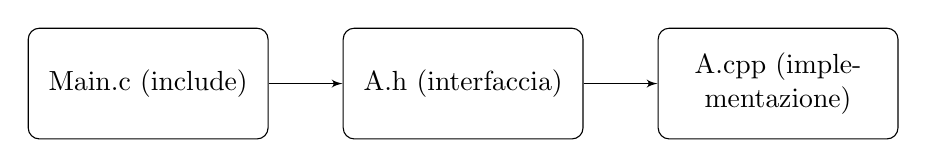
\begin{tikzpicture}[node distance=1cm]
                \node [focus] at (0,0) (main) {Main.c (include)};
                \node [focus] at (4,0) (header) {A.h (interfaccia)};
                \node [focus] at (8,0) (impl) {A.cpp (implementazione)};
                \path [line] (main) -- (header);
                \path [line] (header) -- (impl);
            \end{tikzpicture}
            \caption{Utilizzo di un modulo}
        \end{center}    
    \end{figure}
    Un programma in C++ consiste in piú file sorgente compilati separatamente in file oggetto, successivamente collegati da un "linker", che produce la forma eseguibile del programma
    \begin{figure}[h]
            \begin{center}
            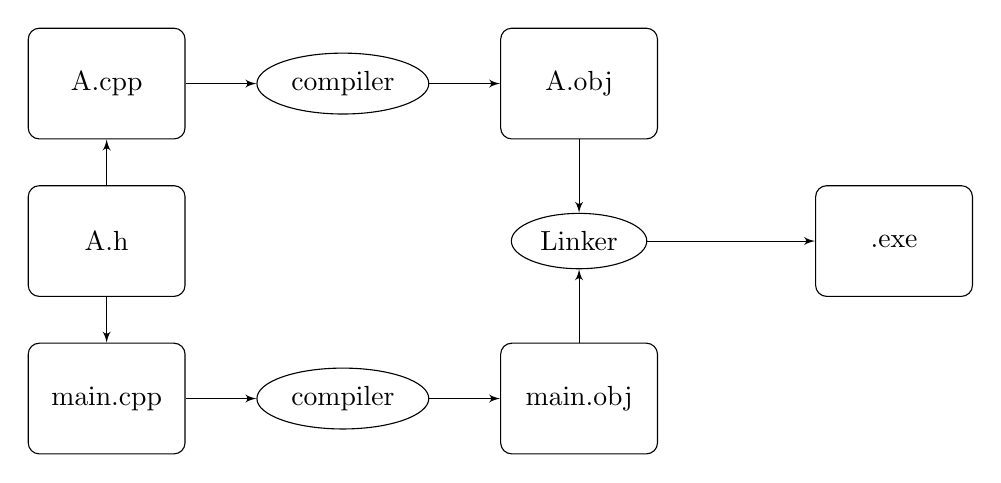
\begin{tikzpicture}[node distance=1cm]
                \node [block] at (0,0) (maincpp) {main.cpp};
                \node [cloud] at (3,0) (compiler1) {compiler};
                \node [block] at (6,0) (mainobj) {main.obj};
                \node [block] at (0,2) (ah) {A.h};
                \node [block] at (0,4) (Acpp) {A.cpp};
                \node [cloud] at (3,4) (compiler2) {compiler};
                \node [block] at (6,4) (Aobj) {A.obj};
                \node [cloud] at (6,2) (linker) {Linker};
                \node [block] at (10,2) (exe) {.exe};
                \path [line] (maincpp) -- (compiler1);
                \path [line] (compiler1) -- (mainobj);
                \path [line] (Acpp) -- (compiler2);
                \path [line] (compiler2) -- (Aobj);
                \path [line] (ah) -- (maincpp);
                \path [line] (ah) -- (Acpp);
                \path [line] (Aobj) -- (linker);
                \path [line] (mainobj) -- (linker);
                \path [line] (linker) -- (exe);
            \end{tikzpicture}
            \caption{Compilazione separata}
        \end{center}    
  \end{figure}
  \subsection{Inclusione di file}
  In C, il preprocessore tramite la direttiva \textbf{include}, puó ricercare il file indicato in alcune directory standard o definite al momento della compilazione ed espanderlo testualmente in sostituzione della direttiva. In C la direttiva include si applica in due diverse forme
  \begin{lstlisting}[language=c]
    #include <nome-file>
    #include "nome-file"
  \end{lstlisting}
  \begin{itemize}
    \item Nel primo caso, il nomefile viene ricercato nelle directory standard definite dall'implementazione ed in altre che sono specificate al momento della compilazione
    \item Nel secondo caso, il nomefile viene ricercato nella directory corrente, e successivamente se non viene trovato, nelle directory standard e quelle specificate al momento della compilazione come nel primo caso
  \end{itemize}
\section{Operazioni su File}
\subsection{Stream}
Il sistema di I/O di C e C++ si basa sul concetto di stream. Per stream, si intende un flusso di dati (sorgente o destinazione) che puó essere associato ad una periferica o alla stessa maniera ad un file proveniente dalla memoria di massa. \\ 
In altre parole uno stream é un interfaccia comune a diversi dispositivi di I/O che permette di:
\begin{itemize}
  \item rendere la scrittura dei programmi indipendenti dal particolare dispositivo impiegato
  \item Semplificare i problemi di portabilitá dei programmi. 
\end{itemize}
Lo stream consente di definire un'interfaccia semplice di astrazione di un dispositivo generico e uniforme verso l'utente
\subsubsection{Tipi di stream}
La libreria dedicata alle operazione su gli stream, sia in c che in c++ supporta stream di testo e stream binari.
\begin{itemize}
  \item Uno stream di \textbf{testo} é una sequenza di linee, ciascuna formata da caratteri e chiusa dal carattere "$\backslash$ n"
    Uno stream \textbf{binario} é una sequenza di byte, che registrano dati interni (di qualsiasi tipo) chiusa da un terminatore \textbf{end-of-file} garantendo che esista corrispondenza tra quello che viene scritto e successivamente letto sullo stesso sistema
\end{itemize}
\subsubsection{Connessione di uno stream}
Nel caso di operazioni di I/O verso un \textbf{dispositivo}, lo stream viene connesso tramite una operazione di apertura,ossia viene creato un oggetto e linkato ad uno stream.
La connessione viene interrotta con un'operazione di chiusura, e possiamo definire due operazioni sullo stream:
\begin{itemize}
  \item \textbf{Estrazione da un flusso}: la ricezione di dati da un dispositivo di input
  \item \textbf{Inserimento in un flusso}: la trasmissione di dati ad un dispositivo di uscita
\end{itemize}
Nel caso di operazioni di I/O verso la \textbf{memoria di massa}, sia ha una generalizzazione delle operazioni primarie. Ad esempio in C e C++ la libreria I/O mette a disposizione tre classi
\begin{itemize}
  \item \textbf{ifstream}: operazioni di input
  \item \textbf{ofstream}: operazioni di output
  \item \textbf{fstream}: operazioni di aggiornamento
\end{itemize}
\subsubsection{Stream standard di I/O}
In C++ un programma comunica con l'esterno mediante i seguenti stream standard
\begin{itemize}
  \item \textbf{stdin}: standard input (associato di default alla tastiera)
  \item \textbf{stdout}: standard output (associato di default al video)
  \item \textbf{stderr}: standard output per i messaggi (associato al video)
\end{itemize}
Gli stream sovraelencati sono rappresentamente il canale di immissione dati, uscita dei risultati, riporto delle eventuali situazioni di errore. Questi stream sono collegati alle variabili globali cin, cout, cerr, e si possono utilizzare attraverso gli \textbf{operatori di flusso} "$>>$" (estrazione) e "$<<$" (inserimento).
\subsection{File}
Per memorizzare un dato su un'unità di memoria di massa viene utilizzata una variabile di tipo stream chiamata \textbf{File}. Esistono due varianti
\begin{itemize}
  \item \textbf{File di testo}: Una sequenza di caratteri che durante il trasferimento può subire conversioni a seconda delle necessità e dell'ambiente di destinazione 
  \item \textbf{File binari}: una sequenza di Byte
\end{itemize}
\subsubsection{Posizionamento in lettura e scrittura}
La libreria fstream gestisce due puntatori, uno per la lettura e uno per la scrittura che possono essere riposizionati usando le funzioni apposite
\begin{itemize}
\item Posizionamento e interrogazione del puntatore in lettura: 
  \begin{lstlisting}[language=c]
    seekg() //
    tellg() //
  \end{lstlisting}
\item Posizionamento e interrogazione del puntatore in scrittura: 
  \begin{lstlisting}[language=c]
    seekp() //
    tellp() //
  \end{lstlisting}
\end{itemize}













\end{document}
